% generated by scripts/pkl_to_latex.py
% source PKL : vscan_v1_L8_Ne8_U10_t1_mode-uniform_nmin2_solver-gcg_full_restarts10_iter300_kmax5_tol1em09_V0to12_N25-ebabade1a2a1.pkl
% scan type  : vscan
% state      : gs
% quantity   : linear-entropy
% requires   : \usepackage{pgfplots} \pgfplotsset{compat=1.18}
% colours match the matplotlib PDF (tab10 cycle)
\definecolor{gmeC0}{HTML}{1F77B4}
\definecolor{gmeC1}{HTML}{FF7F0E}
\definecolor{gmeC2}{HTML}{2CA02C}
\definecolor{gmeC3}{HTML}{D62728}
\definecolor{gmeC4}{HTML}{9467BD}
\definecolor{gmeC5}{HTML}{8C564B}
\definecolor{gmeC6}{HTML}{E377C2}
\definecolor{gmeC7}{HTML}{17BECF}

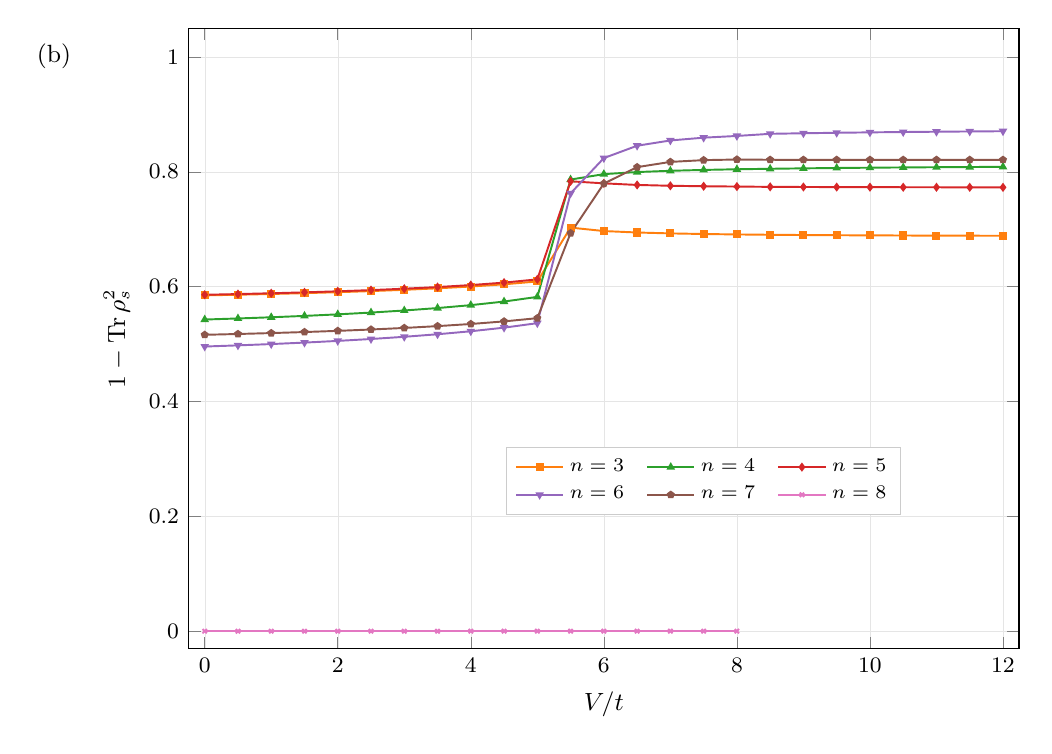
\begin{tikzpicture}
  \begin{axis}[
    width=\columnwidth,
    height=0.78\columnwidth,
    xlabel={$V/t$},
    ylabel={$1-\mathrm{Tr}\,\rho_s^2$},
    grid=both,
    grid style={line width=.1pt, draw=gray!20},
    tick label style={font=\footnotesize\rmfamily, /pgf/number format/fixed},
    label style={font=\small\rmfamily},
    scaled ticks=false,
    legend style={font=\scriptsize\rmfamily, draw=gray!40, at={(0.5,1.03)}, anchor=south, /tikz/every even column/.append style={column sep=6pt}},
    legend cell align={left},
    legend columns=3,
    ymin=-0.03,
    ymax=1.05,
    xmin=-0.24,
    xmax=12.24,
    legend style={at={(0.620,0.270)}, anchor=center, fill=white},
    after end axis/.append code={\node[anchor=east, font=\small\rmfamily] at (axis description cs:-0.13,0.954) {(b)};},
  ]
    \addplot[color=gmeC1, mark=square*, mark size=1.1pt, line width=0.7pt] coordinates {
        (0,0.584753) (0.5,0.585893) (1,0.58718) (1.5,0.58864)
        (2,0.590306) (2.5,0.592222) (3,0.594445) (3.5,0.597056)
        (4,0.600181) (4.5,0.60403) (5,0.609025) (5.5,0.702777)
        (6,0.696789) (6.5,0.694246) (7,0.69269) (7.5,0.691629)
        (8,0.690865) (8.5,0.690291) (9,0.689857) (9.5,0.689517)
        (10,0.689245) (10.5,0.689024) (11,0.688843) (11.5,0.688692)
        (12,0.688565)
    };
    \addlegendentry{$n=3$}
    \addplot[color=gmeC2, mark=triangle*, mark size=1.1pt, line width=0.7pt] coordinates {
        (0,0.542696) (0.5,0.544549) (1,0.546641) (1.5,0.549014)
        (2,0.551722) (2.5,0.554834) (3,0.558443) (3.5,0.562683)
        (4,0.567757) (4.5,0.574012) (5,0.582132) (5.5,0.786459)
        (6,0.795916) (6.5,0.799533) (7,0.801707) (7.5,0.803232)
        (8,0.804384) (8.5,0.805211) (9,0.805967) (9.5,0.806592)
        (10,0.807117) (10.5,0.807566) (11,0.807953) (11.5,0.808292)
        (12,0.808591)
    };
    \addlegendentry{$n=4$}
    \addplot[color=gmeC3, mark=diamond*, mark size=1.1pt, line width=0.7pt] coordinates {
        (0,0.585809) (0.5,0.587046) (1,0.588444) (1.5,0.590033)
        (2,0.591849) (2.5,0.593942) (3,0.596378) (3.5,0.599251)
        (4,0.602709) (4.5,0.607004) (5,0.612641) (5.5,0.783397)
        (6,0.779852) (6.5,0.777071) (7,0.775634) (7.5,0.774794)
        (8,0.774251) (8.5,0.773744) (9,0.77352) (9.5,0.773347)
        (10,0.77321) (10.5,0.773102) (11,0.773014) (11.5,0.772943)
        (12,0.772885)
    };
    \addlegendentry{$n=5$}
    \addplot[color=gmeC4, mark=triangle*, mark size=1.1pt, mark options={rotate=180}, line width=0.7pt] coordinates {
        (0,0.495677) (0.5,0.4977) (1,0.499977) (1.5,0.502549)
        (2,0.505467) (2.5,0.508796) (3,0.512621) (3.5,0.517056)
        (4,0.522271) (4.5,0.528542) (5,0.536388) (5.5,0.762448)
        (6,0.823847) (6.5,0.845359) (7,0.854543) (7.5,0.859401)
        (8,0.862395) (8.5,0.866098) (9,0.867093) (9.5,0.867926)
        (10,0.868633) (10.5,0.86924) (11,0.869767) (11.5,0.870228)
        (12,0.870636)
    };
    \addlegendentry{$n=6$}
    \addplot[color=gmeC5, mark=pentagon*, mark size=1.1pt, line width=0.7pt] coordinates {
        (0,0.516106) (0.5,0.517518) (1,0.519111) (1.5,0.520917)
        (2,0.522973) (2.5,0.525327) (3,0.528044) (3.5,0.531208)
        (4,0.534943) (4.5,0.539447) (5,0.545085) (5.5,0.693114)
        (6,0.779409) (6.5,0.808091) (7,0.817196) (7.5,0.82028)
        (8,0.821363) (8.5,0.820896) (9,0.820875) (9.5,0.820859)
        (10,0.820848) (10.5,0.82084) (11,0.820835) (11.5,0.820833)
        (12,0.820832)
    };
    \addlegendentry{$n=7$}
    \addplot[color=gmeC6, mark=x, mark size=1.1pt, line width=0.7pt] coordinates {
        (0,0) (0.5,0) (1,-0) (1.5,-0)
        (2,-0) (2.5,0) (3,0) (3.5,-0)
        (4,-0) (4.5,0) (5,0) (5.5,-0)
        (6,-0) (6.5,-0) (7,-0) (7.5,0)
        (8,-0)
    };
    \addlegendentry{$n=8$}
  \end{axis}
\end{tikzpicture}
